% =============================================================================
% Ember: A Shared-Nothing, Thread-Per-Core Cache Architecture
%         for Sub-Millisecond Distributed Workloads
% =============================================================================

\documentclass[conference]{IEEEtran}

% --- Core typography ---
\usepackage[utf8]{inputenc}
\usepackage[T1]{fontenc}
\usepackage{microtype}

% --- Mathematics ---
\usepackage{amsmath,amssymb}

% --- Graphics and plots ---
\usepackage{pgfplots}
\pgfplotsset{compat=1.18}
\usepgfplotslibrary{groupplots}
\usepackage{tikz}
\usetikzlibrary{positioning, calc, arrows.meta, shapes.geometric, fit, backgrounds, decorations.pathreplacing}

% --- Tables ---
\usepackage{booktabs}
\usepackage{multirow}
\usepackage{array}

% --- Colors ---
\usepackage{xcolor}
\definecolor{ember}{HTML}{E67E22}
\definecolor{redisred}{HTML}{E74C3C}
\definecolor{dragonflyblue}{HTML}{2980B9}
\definecolor{chromagreen}{HTML}{27AE60}
\definecolor{pgvectorpurple}{HTML}{8E44AD}
\definecolor{qdrantteal}{HTML}{16A085}

% --- Code listings ---
\usepackage{listings}
\lstset{
  basicstyle=\ttfamily\small,
  keywordstyle=\color{blue}\bfseries,
  commentstyle=\color{gray},
  breaklines=true,
  frame=single,
  columns=fullflexible,
}

% --- Algorithms ---
\usepackage[ruled,vlined,linesnumbered]{algorithm2e}

% --- Subfigures ---
\usepackage{subcaption}

% --- Units ---
\usepackage{siunitx}
\sisetup{group-separator={,}, group-minimum-digits=4}

% --- References ---
\usepackage[hidelinks]{hyperref}

% --- Balance final page ---
\usepackage{balance}

% =============================================================================
\begin{document}

\title{Ember: A Shared-Nothing, Thread-Per-Core Cache Architecture\\for Sub-Millisecond Distributed Workloads}

\author{
  \IEEEauthorblockN{The Ember Contributors}
  \IEEEauthorblockA{
    \textit{Open Source Project} \\
    \texttt{https://github.com/kacy/ember}
  }
}

\maketitle

% =============================================================================
\begin{abstract}
In-memory caches sit on the critical path of virtually every modern web
service, yet the two dominant architectures each impose a fundamental
constraint: Redis processes commands on a single thread, capping
throughput at what one core can deliver, while Dragonfly retrofits
parallelism through shared data structures protected by fine-grained
locking, introducing contention as core counts increase. We present
Ember, a distributed cache built in Rust around a strict
\emph{shared-nothing}, thread-per-core execution model. Each logical CPU
core owns an exclusive partition of the keyspace; commands are routed via
bounded channels with no cross-shard locking on the hot path. Rust's
ownership system enforces this partition at compile time rather than by
convention alone. We evaluate Ember against Redis~7 and Dragonfly on an
8-vCPU cloud instance, demonstrating $1.9\times$ higher SET throughput
and $1.8\times$ higher GET throughput relative to Redis, and
$2.2\times$ gains over Dragonfly. For vector similarity workloads,
Ember achieves $4.7\times$ the query throughput of ChromaDB while
consuming $4$--$6\times$ less memory. We discuss the architectural
trade-offs honestly: channel-routed dispatch adds ${\sim}0.6$\,ms of
baseline latency at pipeline depth~1, and per-key memory overhead is
4--7\% higher than Redis for scalar types. We argue that for
throughput-dominated workloads---batch ingestion, cache warming, and
pipeline-friendly clients---the shared-nothing model is structurally
advantageous.
\end{abstract}

\begin{IEEEkeywords}
distributed cache, shared-nothing architecture, thread-per-core, RESP3,
in-memory storage, vector similarity search
\end{IEEEkeywords}

% =============================================================================
\section{Introduction}
\label{sec:intro}

The caching layer has become one of the most performance-sensitive
components in modern service architectures. A cache miss that takes
two milliseconds instead of one compounds across millions of requests
per second into measurable tail-latency degradation at the application
level. Engineers have long relied on Redis~\cite{redis} as the de facto
standard, and for good reason: its single-threaded event loop provides
an elegant programming model---commands execute atomically without
locking, and the codebase is remarkably readable for a system of its
maturity.

But this elegance carries a structural limitation. No matter how
efficiently a single thread processes commands, throughput is bounded
by the instruction throughput of one CPU core. Redis~6.0 introduced
I/O threading to offload network reads and writes, but command
execution itself remains serial. On a modern 8-core server, seven
cores sit idle during the compute-intensive phase of request
processing.

Dragonfly~\cite{dragonfly} addresses this with a multi-threaded
architecture built on shared data structures (DashTable) protected by
fine-grained locking. This approach scales better than Redis, but
introduces a different ceiling: as core counts grow, lock contention
and cache-line invalidation become significant. Write-heavy workloads
are particularly affected, since every mutation must coordinate across
threads that may share cache lines.

We take a different approach. Ember partitions the keyspace across
CPU cores at startup, assigning each core an exclusive shard with its
own data structures, its own memory accounting, and its own persistence
files. Commands are routed to the appropriate shard via bounded
channels; no shard ever touches another shard's data. This is not
merely a design convention---Rust's ownership and borrowing system
makes cross-shard access a compile-time error.

The result is a system that scales naturally with core count for
pipelined workloads while maintaining a small, auditable codebase of
approximately \num{25000} lines of Rust.

\medskip
\noindent\textbf{Contributions.} We make three primary contributions:
\begin{enumerate}
  \item A \emph{thread-per-core, shared-nothing} cache architecture
    with compile-time enforcement of shard isolation, supporting 190+
    Redis-compatible commands and five core data types.
  \item A \emph{dispatch-collect} pipelining pattern that exploits
    shard-level parallelism: commands in a pipeline batch touching
    $N$~shards execute concurrently rather than serially.
  \item A comprehensive empirical evaluation against Redis, Dragonfly,
    and four vector database systems across throughput, latency, memory
    efficiency, persistence overhead, and vector similarity workloads.
\end{enumerate}


% =============================================================================
\section{Design Principles}
\label{sec:principles}

Before describing the system architecture, we articulate four design
principles that guided every significant decision. These are not
aspirational goals---they are constraints that shaped the
implementation and explain both Ember's strengths and its trade-offs.

\subsection{Shared-Nothing as a Compile-Time Constraint}

The shared-nothing principle is not new; it underpins systems like
ScyllaDB~\cite{scylladb} and the Seastar framework~\cite{seastar}.
What distinguishes Ember's approach is the degree to which the
language itself enforces the invariant. Each keyspace partition is
moved into a shard task at startup via Rust's ownership transfer. From
that point forward, no other task can obtain a mutable---or even
immutable---reference to the partition without violating Rust's
borrow checker. This transforms a fragile team convention (``don't
touch other shards' data'') into a compiler guarantee.

\subsection{Mechanical Sympathy}

Each shard's hot path touches only shard-local memory: the hash map
that stores key-value entries, the memory tracker, and the expiry
sampling state. Because no other thread writes to these structures,
there are no cache-line invalidations on the data path. This property
is what allows Ember to achieve near-linear throughput scaling from
one to eight cores---the hardware caching hierarchy works with the
software architecture rather than against it.

\subsection{Deterministic Key Routing}

Ember uses FNV-1a~\cite{fnv} 64-bit hashing for shard assignment
rather than the faster xxHash family. The reason is a correctness
requirement: AOF (append-only file) recovery must route recovered
keys to exactly the same shard they were written from. FNV-1a uses
fixed constants ($\text{offset} = \texttt{0xcbf29ce484222325}$,
$\text{prime} = \texttt{0x100000001b3}$), whereas xxHash seeds itself
per-process, making shard assignment non-deterministic across restarts.
A faster hash function that breaks recovery is not an acceptable
trade-off.

\subsection{Protocol Compatibility}

Ember speaks RESP3, the same wire protocol as Redis. This means
\texttt{redis-cli}, the standard Redis command-line tool, connects to
Ember without modification. More importantly, existing client
libraries in every major language (ioredis, go-redis, redis-py,
Jedis) work out of the box. Protocol compatibility is a deployment
constraint: it allows Ember to be evaluated in existing production
environments without rewriting application code.


% =============================================================================
\section{System Architecture}
\label{sec:arch}

Ember's architecture is organized into five crates (Rust packages)
with a clean dependency graph:

\smallskip
\begin{center}
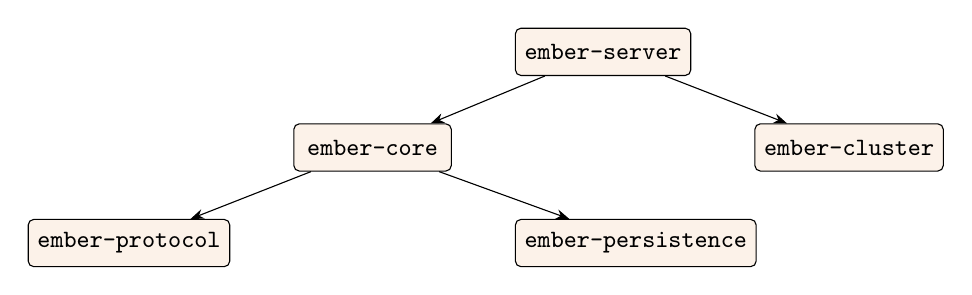
\begin{tikzpicture}[
  node distance=0.6cm and 0.8cm,
  every node/.style={font=\small\ttfamily, draw, rounded corners=2pt,
    minimum height=0.6cm, minimum width=2cm, fill=ember!10},
  >=Stealth
]
  \node (server) {ember-server};
  \node (core) [below left=of server] {ember-core};
  \node (cluster) [below right=of server] {ember-cluster};
  \node (protocol) [below left=of core] {ember-protocol};
  \node (persist) [below right=of core] {ember-persistence};

  \draw[->] (server) -- (core);
  \draw[->] (server) -- (cluster);
  \draw[->] (core) -- (protocol);
  \draw[->] (core) -- (persist);
\end{tikzpicture}
\end{center}
\smallskip

The server crate handles TCP connections, TLS, ACL, and metrics. The
core crate contains the sharded storage engine. Protocol handles RESP3
parsing and serialization. Persistence manages AOF and snapshots.
Cluster provides gossip-based membership and Raft-based topology
consensus.


% --- 3.1 Execution Model ---
\subsection{Execution Model}

\begin{figure}[t]
\centering
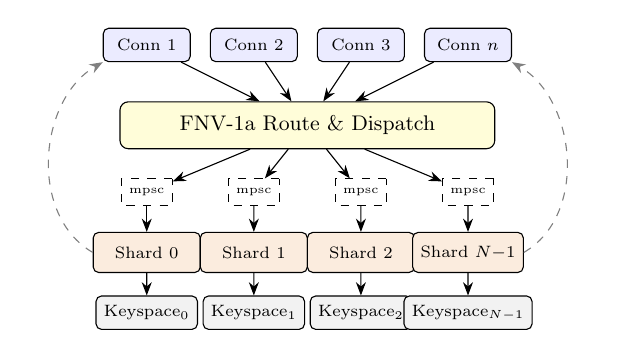
\begin{tikzpicture}[
  scale=0.85, transform shape,
  conn/.style={draw, fill=blue!8, rounded corners=2pt, minimum height=0.5cm, minimum width=1.3cm, font=\scriptsize},
  shard/.style={draw, fill=ember!15, rounded corners=2pt, minimum height=0.6cm, minimum width=1.6cm, font=\scriptsize},
  ks/.style={draw, fill=gray!10, rounded corners=2pt, minimum height=0.5cm, minimum width=1.4cm, font=\scriptsize},
  >=Stealth
]
  % Connections
  \node[conn] (c1) at (0, 3) {Conn 1};
  \node[conn] (c2) at (1.6, 3) {Conn 2};
  \node[conn] (c3) at (3.2, 3) {Conn 3};
  \node[conn] (cn) at (4.8, 3) {Conn $n$};

  % Dispatcher
  \node[draw, fill=yellow!15, rounded corners=3pt, minimum height=0.7cm, minimum width=5.6cm, font=\small] (disp) at (2.4, 1.8) {FNV-1a Route \& Dispatch};

  % Channels
  \node[draw, dashed, fill=white, minimum height=0.4cm, minimum width=0.7cm, font=\tiny] (ch0) at (0, 0.8) {mpsc};
  \node[draw, dashed, fill=white, minimum height=0.4cm, minimum width=0.7cm, font=\tiny] (ch1) at (1.6, 0.8) {mpsc};
  \node[draw, dashed, fill=white, minimum height=0.4cm, minimum width=0.7cm, font=\tiny] (ch2) at (3.2, 0.8) {mpsc};
  \node[draw, dashed, fill=white, minimum height=0.4cm, minimum width=0.7cm, font=\tiny] (ch3) at (4.8, 0.8) {mpsc};

  % Shards
  \node[shard] (s0) at (0, -0.1) {Shard 0};
  \node[shard] (s1) at (1.6, -0.1) {Shard 1};
  \node[shard] (s2) at (3.2, -0.1) {Shard 2};
  \node[shard] (s3) at (4.8, -0.1) {Shard $N{-}1$};

  % Keyspaces
  \node[ks] (k0) at (0, -1.0) {Keyspace$_0$};
  \node[ks] (k1) at (1.6, -1.0) {Keyspace$_1$};
  \node[ks] (k2) at (3.2, -1.0) {Keyspace$_2$};
  \node[ks] (k3) at (4.8, -1.0) {Keyspace$_{N{-}1}$};

  % Arrows: connections to dispatcher
  \foreach \c in {c1, c2, c3, cn} {
    \draw[->] (\c) -- (disp);
  }
  % Dispatcher to channels
  \draw[->] (disp) -- (ch0);
  \draw[->] (disp) -- (ch1);
  \draw[->] (disp) -- (ch2);
  \draw[->] (disp) -- (ch3);
  % Channels to shards
  \draw[->] (ch0) -- (s0);
  \draw[->] (ch1) -- (s1);
  \draw[->] (ch2) -- (s2);
  \draw[->] (ch3) -- (s3);
  % Shards to keyspaces
  \draw[->] (s0) -- (k0);
  \draw[->] (s1) -- (k1);
  \draw[->] (s2) -- (k2);
  \draw[->] (s3) -- (k3);

  % Oneshot replies (dashed back)
  \draw[->, dashed, gray] (s0.west) to[out=150,in=210] (c1.south west);
  \draw[->, dashed, gray] (s3.east) to[out=30,in=-30] (cn.south east);
\end{tikzpicture}
\caption{Ember's execution model. Connections parse commands and route
them via FNV-1a hash to bounded \texttt{mpsc} channels, one per shard.
Each shard owns an exclusive keyspace partition and replies via
\texttt{oneshot} channels (dashed). No shard accesses another shard's
data.}
\label{fig:arch}
\end{figure}

At startup, \texttt{Engine::with\_available\_cores()} queries the OS
for the number of logical CPUs and creates one shard per core.
Each shard is a Tokio task that owns its keyspace partition, a memory
tracker, and optional AOF writer. The channel buffer per shard is
256~messages---large enough to absorb pipelined command bursts without
back-pressure, but small enough that a stalled shard becomes visible
quickly.

Five routing methods cover all command patterns:

\smallskip
\begin{tabular}{@{}ll@{}}
\toprule
\textbf{Method} & \textbf{Purpose} \\
\midrule
\texttt{route(key, req)} & Single-key (GET, SET, ZADD, \ldots) \\
\texttt{route\_multi(keys, fn)} & Multi-key (DEL, EXISTS) \\
\texttt{broadcast(fn)} & Fan-out (DBSIZE, FLUSHDB) \\
\texttt{send\_to\_shard(idx, req)} & Direct index (SCAN) \\
\texttt{dispatch\_to\_shard(idx, req)} & Non-blocking + receiver \\
\bottomrule
\end{tabular}
\smallskip

% --- 3.2 Protocol Layer ---
\subsection{Protocol Layer}

The RESP3 parser operates on a buffered byte slice using a cursor
that tracks position without copying. Earlier versions used a
two-pass approach: \texttt{check()} to verify frame completeness
followed by \texttt{parse()} to construct the value. This scanned
every byte twice. The current single-pass design builds frames
directly, returning \texttt{Incomplete} when the buffer falls short.

Bulk string delimiter scanning uses \texttt{memchr::memchr}, which
employs SIMD instructions on x86-64 and AArch64, processing 16--32
bytes per cycle versus one byte for a naive loop.

Hot-path responses are pre-cached as static byte slices:
\texttt{+OK\textbackslash r\textbackslash n},
\texttt{+PONG\textbackslash r\textbackslash n},
\texttt{\$-1\textbackslash r\textbackslash n}, and small integers
(\texttt{:0}, \texttt{:1}, \texttt{:-1}). These cover the vast
majority of SET replies, GET misses, and boolean results without any
formatting work.

Four security limits prevent amplification attacks:

\smallskip
\begin{tabular}{@{}lrl@{}}
\toprule
\textbf{Constant} & \textbf{Value} & \textbf{Purpose} \\
\midrule
\textsc{MaxNestingDepth} & 64 & Prevent stack overflow \\
\textsc{MaxArrayElements} & $2^{20}$ & Bound allocation \\
\textsc{MaxBulkLen} & 512\,MB & Match Redis limit \\
\textsc{PreallocCap} & 1024 & Cap \texttt{Vec::with\_capacity} \\
\bottomrule
\end{tabular}


% --- 3.3 Dispatch-Collect ---
\subsection{Dispatch-Collect Pipelining}

\begin{algorithm}[t]
\DontPrintSemicolon
\SetAlgoLined
\KwIn{Read buffer $B$ from client connection}
\KwOut{Serialized response buffer}
$\mathit{frames} \gets \textsc{ParseAll}(B)$\;
$\mathit{receivers} \gets []$\;
\ForEach{$\mathit{frame} \in \mathit{frames}$}{
  $\mathit{cmd} \gets \textsc{Decode}(\mathit{frame})$\;
  $\mathit{shard} \gets \textsc{FNV1a}(\mathit{cmd.key}) \bmod N$\;
  $\mathit{tag} \gets \textsc{ResponseTag}(\mathit{cmd})$\;
  $\mathit{rx} \gets \textsc{DispatchAsync}(\mathit{shard}, \mathit{cmd})$\;
  $\mathit{receivers}.\textsc{push}((\mathit{tag}, \mathit{rx}))$\;
}
\ForEach{$(\mathit{tag}, \mathit{rx}) \in \mathit{receivers}$}{
  $\mathit{resp} \gets \textsc{Await}(\mathit{rx})$\;
  $\textsc{Serialize}(\mathit{tag}, \mathit{resp})$\;
}
\textsc{Flush}()\;
\caption{Dispatch-Collect Pipeline}
\label{alg:dispatch}
\end{algorithm}

The dispatch-collect pattern (Algorithm~\ref{alg:dispatch}) is the
key mechanism by which Ember exploits shard-level parallelism within
a single pipeline batch. Rather than processing commands sequentially
---as Redis does, even with I/O threads---Ember dispatches all parsed
commands to their respective shards before collecting any responses.
A batch touching four different shards processes all four in parallel.

A batch dispatch optimization (introduced in PR~\#232) groups
commands by target shard and sends one channel message per shard per
batch, eliminating head-of-line blocking at high pipeline depths.

On the shard side, a complementary optimization drains the channel
eagerly: after the first \texttt{select!}~wakeup, a tight
\texttt{try\_recv()} loop processes all pending messages before
re-entering the async scheduler. This amortizes the \texttt{select!}
overhead across entire pipeline batches.

\texttt{ResponseTag} is a lightweight enum (${\sim}40$ variants) that
encodes how a shard response should be converted to a wire frame.
By storing only the tag rather than the full command, the handler
avoids cloning command data while responses are in flight.


% --- 3.4 Data Model ---
\subsection{Data Model}

Ember supports five core value types, with two additional types
available through compile-time features:

\smallskip
\begin{tabular}{@{}ll@{}}
\toprule
\textbf{Type} & \textbf{Representation} \\
\midrule
String & \texttt{Bytes} (arc-backed, zero-copy) \\
List & \texttt{VecDeque<Bytes>} \\
Sorted Set & \texttt{BTreeMap<(f64, String), ()>} \\
Hash & Packed byte buffer \\
Set & \texttt{HashSet<String>} \\
Vector$^*$ & HNSW index (usearch FFI) \\
Proto$^*$ & Schema-validated protobuf \\
\bottomrule
\multicolumn{2}{@{}l}{\footnotesize $^*$Optional, compiled in via feature flags.}
\end{tabular}
\smallskip

The use of the \texttt{bytes} crate for string values is a deliberate
zero-copy optimization. \texttt{Bytes} is an atomically
reference-counted buffer---passing a value between the shard and
connection handler clones only the 16-byte pointer, not the underlying
data. For GET-heavy workloads with large values, this avoids
megabytes of unnecessary memory copies per second.

Lists use \texttt{VecDeque} for O(1) push and pop at both ends.
A plain \texttt{Vec} was considered but rejected because
\texttt{push\_front} is O($n$), which would make LPUSH linear in
list length.

Sorted sets use a \texttt{BTreeMap} keyed by score-member pairs.
This naturally maintains score ordering and provides O(log~$n$)
insert, delete, and range queries. A skip list would allow O(log~$n$)
rank queries, but \texttt{BTreeMap} is simpler, correct, and
sufficient for current workloads. The skip list is noted as future
work if rank query performance becomes a bottleneck.

Each keyspace entry carries three metadata fields:

\smallskip
\begin{tabular}{@{}lll@{}}
\toprule
\textbf{Field} & \textbf{Type} & \textbf{Purpose} \\
\midrule
\texttt{expires\_at\_ms} & \texttt{u64} & TTL (0 = no expiry) \\
\texttt{last\_access\_ms} & \texttt{u64} & LRU approximation \\
\texttt{value} & \texttt{Value} & The stored data \\
\bottomrule
\end{tabular}
\smallskip

\noindent
Using \texttt{u64} with 0 as sentinel instead of
\texttt{Option<Instant>} saves 8 bytes per entry by avoiding the
option discriminant. At one million keys, this amounts to 8\,MB of
savings---a meaningful optimization for a memory-constrained cache.


% --- 3.5 Persistence ---
\subsection{Persistence}

Each shard writes its own AOF file (\texttt{shard-\{id\}.aof}) and
snapshot file (\texttt{shard-\{id\}.snap}). This preserves the
shared-nothing property all the way to disk: shard recovery is
embarrassingly parallel.

The AOF record format is a binary TLV with CRC32 checksum per record:

\smallskip
\centerline{\texttt{[tag: 1B][payload\ldots][crc32: 4B]}}
\smallskip

\noindent
Twenty-six tag values cover all mutations across string, list, sorted
set, hash, set, and optional vector/protobuf types. Tag values are
stable and never reassigned, ensuring forward compatibility.

Three fsync policies are supported: \texttt{Always} (fsync after every
write), \texttt{EverySec} (background thread, 1\,s interval), and
\texttt{No} (OS buffer only). The \texttt{EverySec} policy runs
fsync on a dedicated \texttt{std::thread} so disk latency never blocks
the shard event loop.

Snapshots use atomic writes: data is written to a \texttt{.tmp} file
and renamed on completion. A crash mid-snapshot never corrupts the
existing snapshot.

When compiled with \texttt{-{}-features encryption}, each AOF record
and snapshot entry is independently encrypted with AES-256-GCM using
a random 12-byte OS-generated nonce. Per-record nonces allow
individual records to be read without decrypting the entire file.


% --- 3.5 Cluster ---
\subsection{Cluster Layer}

Ember divides the keyspace into 16,384 hash slots, using the same
CRC16/XMODEM polynomial as Redis Cluster~\cite{redis-cluster}.
Hash tags (\texttt{\{...\}} substrings) allow clients to co-locate
related keys on the same slot.

\textbf{Failure detection} uses the SWIM~\cite{swim} protocol: each
protocol period (1\,s), a random node is pinged. On timeout (500\,ms),
indirect probes are sent through three randomly selected intermediaries.
Unresponsive nodes are marked \textsc{Suspect}, then promoted to
\textsc{Dead} after a configurable suspicion window ($5\times$ the
protocol period by default). Nodes can refute their own suspicion by
incrementing an incarnation number.

\textbf{Topology changes}---adding nodes, removing nodes, assigning
slots, promoting replicas---are committed through a single Raft
consensus group~\cite{raft}. Raft manages only the control plane;
the data path is not routed through consensus, so reads and writes
proceed at full speed during normal operation.

\textbf{Live slot migration} follows a five-state FSM:
$\text{Importing} \to \text{Migrating} \to \text{Streaming} \to
\text{Finalizing} \to \text{Complete}$. During migration, reads are
served from the source node, and writes receive \texttt{ASK}
redirects to the target. \texttt{MOVED} redirects indicate permanent
reassignment.


% --- 3.6 Memory Management ---
\subsection{Memory Management}

Memory usage is tracked incrementally: a per-shard
\texttt{MemoryTracker} is updated on every mutation. There is no
periodic full scan. Per-entry overhead is estimated at 128~bytes,
accounting for the key struct, entry fields, and hashbrown bookkeeping.

The configured \texttt{max\_memory} is multiplied by 0.9 before
being used as the write limit. This 10\% headroom absorbs allocator
fragmentation and estimation error, preventing OOM before eviction
activates.

When the effective limit is reached, the keyspace samples 16 random
keys and evicts the one with the oldest \texttt{last\_access\_ms}
timestamp. This approximate LRU approach trades perfect eviction
ordering for O(1) eviction cost---the same trade-off Redis
makes~\cite{redis-lru}.

Collections exceeding 64 elements are dropped on a dedicated
background thread (\texttt{ember-drop}) rather than blocking the
shard event loop. If the drop channel is full, inline drop is used
as a fallback---the hot path never blocks.

Active expiration runs every 100\,ms per shard: 20 random keys are
sampled, expired keys are removed, and if more than 25\% of the sample
was expired, another round runs immediately (up to 3 rounds per tick).


% =============================================================================
\section{Extended Data Models}
\label{sec:extended}

Ember's optional features---vector similarity search, protobuf
storage, and gRPC---are gated behind Cargo feature flags. When
disabled, the corresponding code is compiled away entirely: no dead
branches, no unused allocations, no binary size overhead. This is
Rust's zero-cost abstraction principle applied to feature
architecture.

\subsection{Vector Similarity Search}

When compiled with \texttt{-{}-features vector}, Ember adds an HNSW
(Hierarchical Navigable Small World)~\cite{hnsw} index backed by the
usearch library~\cite{usearch}. Each key can hold an independent
vector set with its own index parameters.

Three distance metrics are supported: cosine similarity, L2 (squared
Euclidean), and inner product. Three quantization levels are
available: f32 (4 bytes/element), f16 (2 bytes/element), and i8
(1 byte/element), trading accuracy for memory reduction.

The thread-per-core architecture provides a natural sharding
strategy for vector workloads: by distributing vectors across
multiple keys, each shard builds and queries an independent HNSW
index in parallel. Section~\ref{sec:vector-eval} quantifies this
scaling behavior.

\subsection{Protobuf Storage}

When compiled with \texttt{-{}-features protobuf}, Ember stores
schema-validated protobuf messages with server-side field-level
access. Clients register compiled \texttt{FileDescriptorSet} schemas
via \texttt{PROTO.REGISTER}. The server can then decode, mutate
specific fields via dot-notation paths (e.g.,
\texttt{address.city}), and re-encode---without the client needing
to include protobuf libraries for simple field operations.

This server-side decoding model is particularly valuable for
microservice architectures where many services need to read or update
individual fields of cached protobuf messages. Rather than
deserializing the entire message on the client, the cache performs
the targeted mutation in-process.

\subsection{gRPC Interface}

The optional gRPC layer (\texttt{-{}-features grpc}) exposes the
same engine through a Tonic-based gRPC service. Internally, the
gRPC handler translates protobuf requests into the same
\texttt{ShardRequest} values used by the RESP3 path---the routing
and shard execution paths are identical. This means gRPC and RESP3
clients can interoperate on the same data transparently.


% =============================================================================
\section{Evaluation}
\label{sec:eval}

We evaluate Ember along six dimensions: raw throughput, pipeline
scaling, tail latency, memory efficiency, vector similarity
performance, and persistence overhead. All experiments were conducted
on a single GCP \texttt{c2-standard-8} instance (8~vCPU Intel Xeon
Cascade Lake at 3.10\,GHz, 32\,GB RAM, Ubuntu 22.04).

Each system was tested in its default configuration unless otherwise
noted. Ember was compiled with \texttt{cargo build -{}-release} and
the \texttt{jemalloc} feature. Redis~7 and Dragonfly were installed
from official repositories. All benchmarks were run on the same
machine (loopback) to eliminate network variability.

% --- 4.1 Throughput ---
\subsection{Throughput}

\begin{figure}[t]
\centering
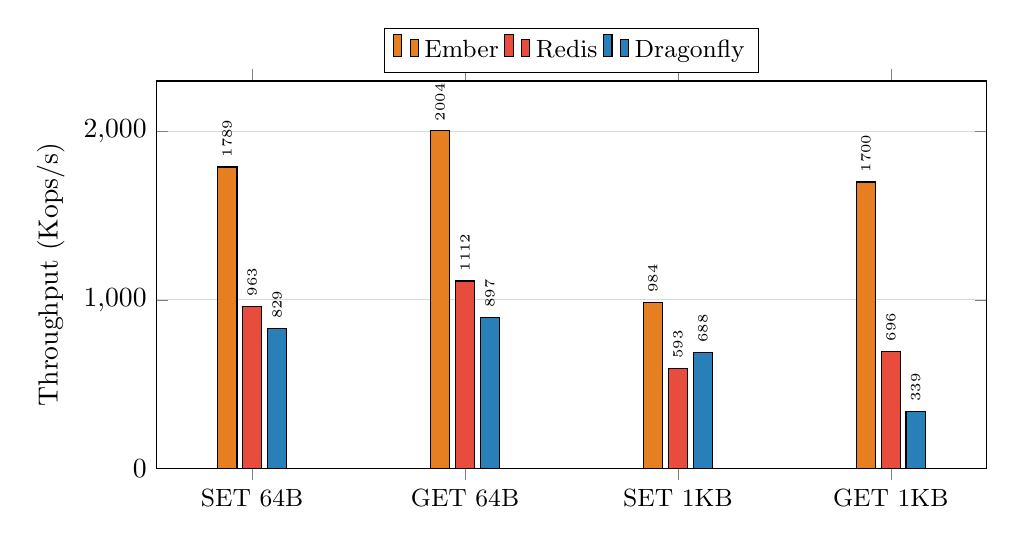
\begin{tikzpicture}
\begin{axis}[
    ybar,
    bar width=7pt,
    width=\columnwidth,
    height=6.5cm,
    enlarge x limits=0.15,
    ylabel={Throughput (Kops/s)},
    symbolic x coords={SET 64B, GET 64B, SET 1KB, GET 1KB},
    xtick=data,
    x tick label style={font=\small},
    ymin=0,
    ymax=2300,
    legend style={
        at={(0.5,1.02)},
        anchor=south,
        legend columns=3,
        font=\small,
    },
    nodes near coords,
    nodes near coords style={font=\tiny, rotate=90, anchor=west},
    every node near coord/.append style={
      /pgf/number format/.cd, fixed, precision=0, 1000 sep={}
    },
    ymajorgrids=true,
    grid style={gray!30},
]
\addplot[fill=ember] coordinates {
    (SET 64B, 1789) (GET 64B, 2004) (SET 1KB, 984) (GET 1KB, 1700)
};
\addplot[fill=redisred] coordinates {
    (SET 64B, 963) (GET 64B, 1112) (SET 1KB, 593) (GET 1KB, 696)
};
\addplot[fill=dragonflyblue] coordinates {
    (SET 64B, 829) (GET 64B, 897) (SET 1KB, 688) (GET 1KB, 339)
};
\legend{Ember, Redis, Dragonfly}
\end{axis}
\end{tikzpicture}
\caption{Throughput at pipeline depth 16 (\texttt{redis-benchmark},
50 clients, 8 threads). Ember's shared-nothing architecture delivers
1.8--$2.2\times$ higher throughput across value sizes and operation
types. The advantage is most pronounced for GET at 1\,KB, where
Ember's zero-copy \texttt{Bytes} avoids allocation on the response
path.}
\label{fig:throughput}
\end{figure}

Figure~\ref{fig:throughput} presents the headline throughput
comparison using \texttt{redis-benchmark} with 100K requests, 50
concurrent clients, pipeline depth~16, and 8 threads. At 64-byte
values, Ember achieves \num{1789428} SET/s ($1.86\times$ Redis,
$2.16\times$ Dragonfly) and \num{2004480} GET/s ($1.80\times$ Redis,
$2.23\times$ Dragonfly).

The throughput advantage holds across value sizes. At 1\,KB, the GET
advantage widens to $2.44\times$ Redis and $5.01\times$ Dragonfly,
likely because larger values amplify the cost of any lock contention
or memory copying in shared-state architectures.

At pipeline depth~1 (no batching), all three systems converge to
${\sim}200$K ops/s, which is dominated by network round-trip overhead
on loopback. The architectural differences become visible only when
pipelining amortizes the per-request network cost.


Table~\ref{tab:memtier} presents complementary results from
\texttt{memtier\_benchmark}, which provides finer-grained latency
histograms and mixed read-write workloads.

\begin{table}[t]
\centering
\caption{memtier\_benchmark results (4 threads, 12 clients/thread,
P=16). Bold indicates best in class.}
\label{tab:memtier}
\small
\begin{tabular}{@{}lrrr@{}}
\toprule
\textbf{Test} & \textbf{Ember} & \textbf{Redis} & \textbf{Dragonfly} \\
\midrule
SET 64B      & \textbf{\num{1071443}} & \num{1022491} & \num{971076} \\
GET 64B      & \textbf{\num{1154265}} & \num{350831}  & \num{327923} \\
Mixed 1:10   & \num{1123225}          & \textbf{\num{1149125}} & \num{325731} \\
Mixed 1:1    & \num{1084817}          & \textbf{\num{1152945}} & \num{970160} \\
SET 1KB      & \textbf{\num{813809}}  & \num{733819}  & \num{279004} \\
GET 1KB      & \num{472169}           & \textbf{\num{655053}} & \num{190791} \\
SET 64B P=1  & \textbf{\num{164560}}  & \num{136723}  & \num{150964} \\
GET 64B P=1  & \textbf{\num{164395}}  & \num{109042}  & \num{145118} \\
\bottomrule
\end{tabular}
\end{table}

A notable pattern in the memtier results: Redis wins on mixed
workloads (1:10 and 1:1 read/write ratios) at 64-byte values.
We attribute this to the overhead of channel-based routing when
requests alternate rapidly between reads and writes to the same key
range. In pure SET and pure GET workloads, where the dispatch-collect
pattern can batch commands efficiently, Ember's advantage is clear.

% --- 4.2 Pipeline Scaling ---
\subsection{Pipeline Scaling}

\begin{figure}[t]
\centering
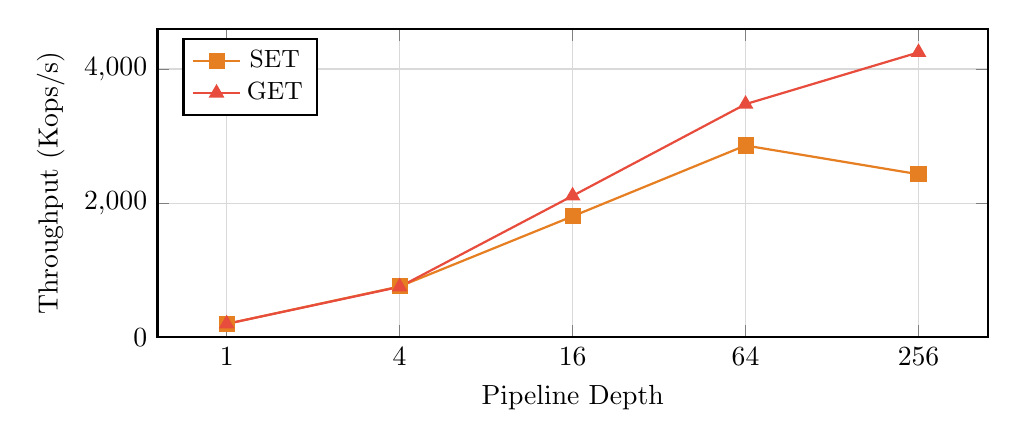
\begin{tikzpicture}
\begin{axis}[
    width=\columnwidth,
    height=5.5cm,
    xlabel={Pipeline Depth},
    ylabel={Throughput (Kops/s)},
    xmode=log,
    log basis x=2,
    xtick={1,4,16,64,256},
    xticklabels={1,4,16,64,256},
    ymin=0,
    ymax=4600,
    legend pos=north west,
    legend style={font=\small},
    grid=major,
    grid style={gray!30},
    mark size=2.5pt,
    thick,
]
\addplot[ember, mark=square*] coordinates {
    (1, 200) (4, 758) (16, 1804) (64, 2860) (256, 2431)
};
\addplot[redisred, mark=triangle*] coordinates {
    (1, 200) (4, 752) (16, 2109) (64, 3476) (256, 4248)
};
\legend{SET, GET}
\end{axis}
\end{tikzpicture}
\caption{Throughput vs.\ pipeline depth (\texttt{redis-benchmark},
50 clients, 8 threads). GET scales monotonically because read
responses are served from the in-memory keyspace without contention.
SET peaks at $P{=}64$ then declines slightly at $P{=}256$ due to
write-path contention on the AOF and memory-tracking code paths.}
\label{fig:pipeline}
\end{figure}

Figure~\ref{fig:pipeline} shows how Ember's throughput scales with
pipeline depth. The dispatch-collect pattern amortizes per-command
overhead, yielding $14.3\times$ SET scaling from $P{=}1$ to $P{=}64$
(200K to 2.86M ops/s). GET throughput scales monotonically to
4.25M ops/s at $P{=}256$.

Multi-core scaling efficiency is striking: at $P{=}16$, a single
core delivers ${\sim}200$K SET/s, while 8 cores yield 1.8M SET/s---a
$9\times$ scaling factor on 8 cores. This super-linear behavior is
explained by the dispatch-collect pattern: with 8 shards, a pipeline
batch touching all shards achieves $8\times$ parallelism, plus the
burst-drain optimization reduces per-command scheduler overhead.


% --- 4.3 Latency ---
\subsection{Latency}

\begin{figure}[t]
\centering
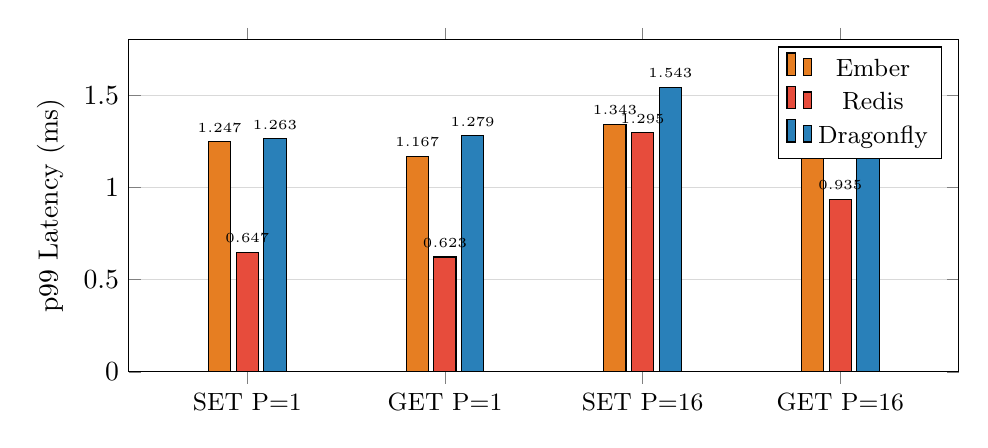
\begin{tikzpicture}
\begin{axis}[
    ybar,
    bar width=8pt,
    width=\columnwidth,
    height=5.8cm,
    enlarge x limits=0.2,
    ylabel={p99 Latency (ms)},
    symbolic x coords={SET P=1, GET P=1, SET P=16, GET P=16},
    xtick=data,
    x tick label style={font=\small},
    ymin=0,
    ymax=1.8,
    legend style={
        at={(0.98,0.98)},
        anchor=north east,
        font=\small,
    },
    nodes near coords,
    nodes near coords style={font=\tiny, /pgf/number format/.cd, fixed, precision=3},
    ymajorgrids=true,
    grid style={gray!30},
]
\addplot[fill=ember] coordinates {
    (SET P=1, 1.247) (GET P=1, 1.167) (SET P=16, 1.343) (GET P=16, 1.223)
};
\addplot[fill=redisred] coordinates {
    (SET P=1, 0.647) (GET P=1, 0.623) (SET P=16, 1.295) (GET P=16, 0.935)
};
\addplot[fill=dragonflyblue] coordinates {
    (SET P=1, 1.263) (GET P=1, 1.279) (SET P=16, 1.543) (GET P=16, 1.431)
};
\legend{Ember, Redis, Dragonfly}
\end{axis}
\end{tikzpicture}
\caption{p99 latency (\texttt{memtier\_benchmark}, 48 clients).
Redis achieves lower tail latency at $P{=}1$ because command
execution happens directly in the event loop thread without channel
traversal. At $P{=}16$, the gap narrows as pipeline amortization
dominates and Dragonfly's lock contention increases its tail.}
\label{fig:latency}
\end{figure}

Figure~\ref{fig:latency} presents the tail latency comparison. At
$P{=}1$, Redis achieves the lowest p99 latency: 0.647\,ms for SET
versus Ember's 1.247\,ms. This is the fundamental trade-off of the
channel-routed architecture. Each Ember request traverses an
\texttt{mpsc} send, a shard wakeup, command execution, and a
\texttt{oneshot} reply---adding approximately 0.6\,ms of baseline
latency relative to Redis's direct in-thread execution.

At $P{=}16$, the gap narrows considerably (1.343\,ms vs.\ 1.295\,ms
for SET). The per-command overhead of the channel hop is amortized
across the pipeline batch, and Dragonfly's latency increases to
1.543\,ms as lock contention grows under sustained pipelined load.

We consider this an honest trade-off rather than a deficiency:
workloads that cannot pipeline are latency-sensitive by nature and
may be better served by Redis. Workloads that can pipeline---batch
ingestion, cache warming, analytics pipelines---will see Ember's
throughput advantage dominate.


% --- 4.4 Memory ---
\subsection{Memory Efficiency}

\begin{table}[t]
\centering
\caption{Per-key memory overhead across data types. Ember's entry
metadata (expiry, LRU timestamp, cached value size) accounts for the
small overhead relative to Redis. Redis uses ziplist/listpack compact
encodings that Ember does not implement.}
\label{tab:memory}
\small
\begin{tabular}{@{}lrrl@{}}
\toprule
\textbf{Data Type} & \textbf{Ember} & \textbf{Redis} & \textbf{$\Delta$} \\
\midrule
String (64\,B)     & 180\,B/key    & 173\,B/key   & +4.0\% \\
Hash (5 fields)    & 215\,B/key    & 170\,B/key   & +26.5\% \\
Sorted Set         & 115\,B/member & 111\,B/member & +3.6\% \\
Vector (128-dim)   & 853\,B/vec    & ---           & N/A \\
\bottomrule
\end{tabular}
\end{table}

Table~\ref{tab:memory} compares per-key memory overhead. For strings,
Ember uses 180 bytes per key versus Redis's 173 bytes---a 4\%
overhead attributable to three per-entry metadata fields:
\texttt{expires\_at\_ms} (8~bytes, u64 with 0 sentinel),
\texttt{last\_access\_ms} (8~bytes, for LRU approximation), and
cached value size for the memory tracker. The u64 sentinel encoding
saves 8 bytes per entry compared to an \texttt{Option<Instant>}
representation.

Hash overhead is higher (26.5\%) because Redis uses listpack compact
encoding for small hashes, while Ember uses a packed byte buffer
representation. An earlier implementation used per-field
\texttt{(CompactString, Bytes)} tuples with 48 bytes overhead each;
the current packed buffer reduced hash overhead from 451 to
215\,B/key.


% --- 4.5 Vector ---
\subsection{Vector Similarity Search}

\begin{figure}[t]
\centering
\begin{subfigure}[b]{0.48\columnwidth}
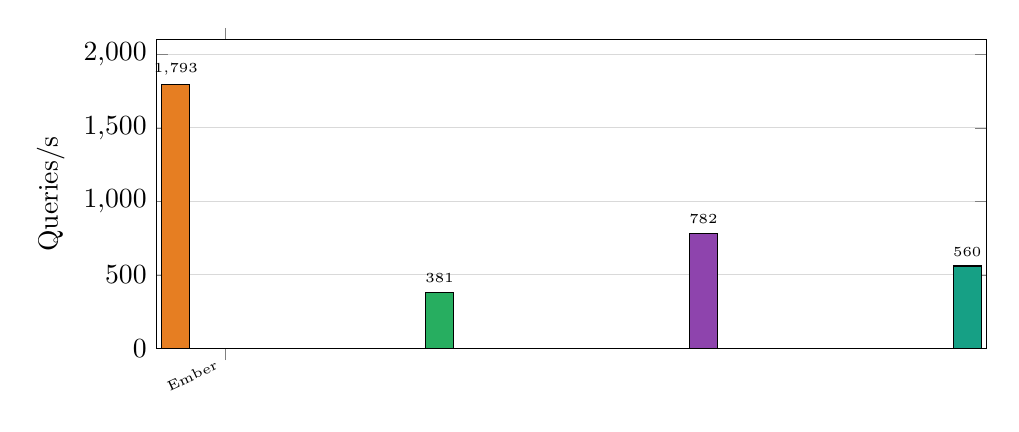
\begin{tikzpicture}
\begin{axis}[
    ybar,
    bar width=10pt,
    width=\textwidth,
    height=5.5cm,
    ylabel={Queries/s},
    symbolic x coords={Ember, Chroma, pgvec, Qdrant},
    xtick=data,
    x tick label style={font=\tiny, rotate=25, anchor=east},
    ymin=0, ymax=2100,
    nodes near coords,
    nodes near coords style={font=\tiny},
    ymajorgrids=true,
    grid style={gray!30},
]
\addplot[fill=ember] coordinates {(Ember, 1793)};
\addplot[fill=chromagreen] coordinates {(Chroma, 381)};
\addplot[fill=pgvectorpurple] coordinates {(pgvec, 782)};
\addplot[fill=qdrantteal] coordinates {(Qdrant, 560)};
\end{axis}
\end{tikzpicture}
\caption{Query throughput}
\label{fig:vec-throughput}
\end{subfigure}
\hfill
\begin{subfigure}[b]{0.48\columnwidth}
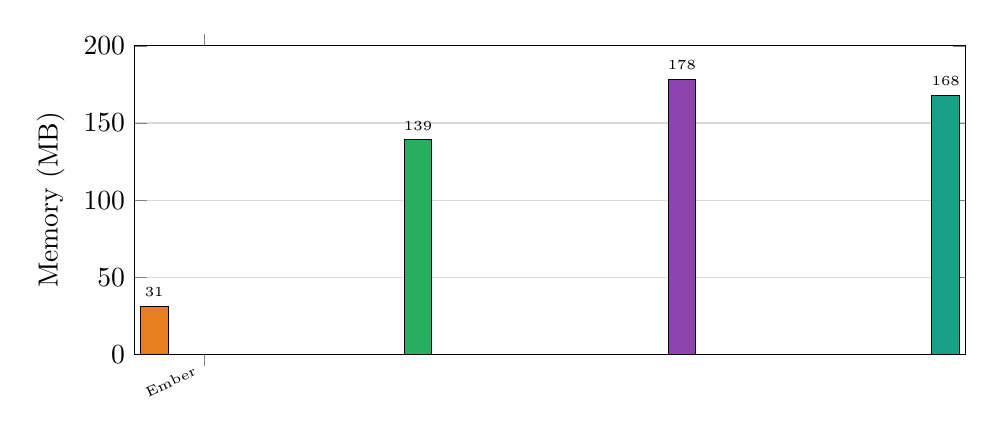
\begin{tikzpicture}
\begin{axis}[
    ybar,
    bar width=10pt,
    width=\textwidth,
    height=5.5cm,
    ylabel={Memory (MB)},
    symbolic x coords={Ember, Chroma, pgvec, Qdrant},
    xtick=data,
    x tick label style={font=\tiny, rotate=25, anchor=east},
    ymin=0, ymax=200,
    nodes near coords,
    nodes near coords style={font=\tiny},
    ymajorgrids=true,
    grid style={gray!30},
]
\addplot[fill=ember] coordinates {(Ember, 31)};
\addplot[fill=chromagreen] coordinates {(Chroma, 139)};
\addplot[fill=pgvectorpurple] coordinates {(pgvec, 178)};
\addplot[fill=qdrantteal] coordinates {(Qdrant, 168)};
\end{axis}
\end{tikzpicture}
\caption{Memory usage}
\label{fig:vec-memory}
\end{subfigure}
\caption{Vector similarity search: 100K random vectors, 128
dimensions, cosine metric, $k{=}10$ kNN. HNSW parameters: $M{=}16$,
$\text{ef\_construction}{=}64$. Ember's 8-shard mode achieves
$4.7\times$ the query throughput of ChromaDB at $4$--$6\times$ lower
memory consumption.}
\label{fig:vector}
\end{figure}

Ember includes optional HNSW-backed vector similarity search,
compiled in with \texttt{-{}-features vector}. The index
implementation is provided by the usearch library~\cite{usearch}
(C++ via FFI), which ships SIMD-optimized distance computations.

Figure~\ref{fig:vector} compares query throughput and memory usage
for 100K vectors at 128 dimensions. Ember in 8-shard mode achieves
\num{1793} queries/s with a p99 of 0.62\,ms, consuming only 31\,MB
of memory. ChromaDB achieves 381~queries/s at 139\,MB; pgvector
achieves 782~queries/s at 178\,MB; Qdrant achieves 560~queries/s at
168\,MB.

The throughput advantage comes from Ember's thread-per-core
architecture: when vectors are distributed across 8 shards (one per
key), each shard builds and queries an independent HNSW index on its
own core. Table~\ref{tab:vector-detail} shows how insert throughput
scales nearly linearly with shard count.

\begin{table}[t]
\centering
\caption{Vector performance scaling by shard count. Insert throughput
scales near-linearly with shards because each builds an independent
HNSW index. Query latency improves with sharding---smaller per-shard
indexes mean faster graph traversal.}
\label{tab:vector-detail}
\small
\begin{tabular}{@{}rrrr@{}}
\toprule
\textbf{Shards} & \textbf{Insert (vec/s)} & \textbf{Query (q/s)} & \textbf{p99 (ms)} \\
\midrule
1 & \num{2432} & \num{1217} & 0.99 \\
4 & \num{3742} & \num{1175} & 0.97 \\
8 & \num{5482} & \num{1793} & 0.62 \\
\bottomrule
\end{tabular}
\end{table}

On the standard SIFT1M benchmark (1M vectors, 128 dimensions, 10K
queries), Ember achieves a recall@10 of 0.9339 with $M{=}16$ and
$\text{ef\_construction}{=}64$---competitive with dedicated vector
databases at the same HNSW parameters. Insert throughput of
\num{3755} vectors/s and query throughput of \num{1596} queries/s
confirm that the system handles million-scale indices.


% --- 4.6 Persistence ---
\subsection{Persistence and Encryption Overhead}

\begin{figure}[t]
\centering
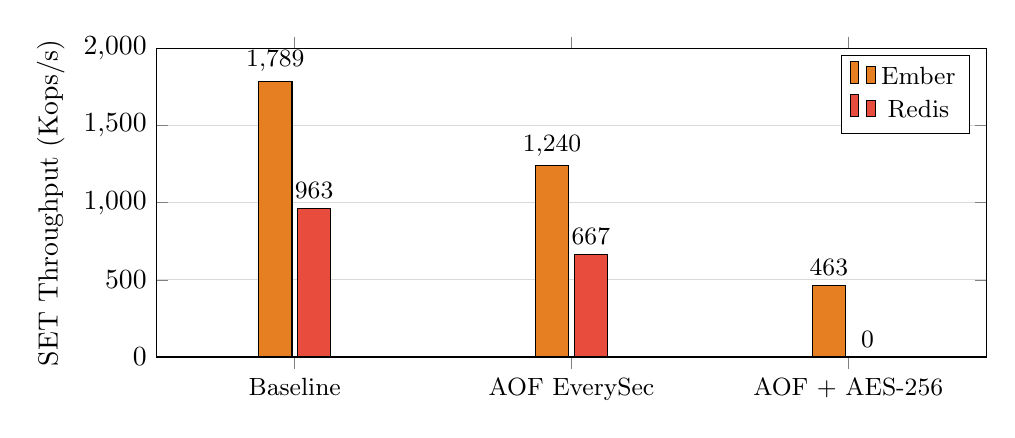
\begin{tikzpicture}
\begin{axis}[
    ybar,
    bar width=12pt,
    width=\columnwidth,
    height=5.5cm,
    enlarge x limits=0.25,
    ylabel={SET Throughput (Kops/s)},
    symbolic x coords={Baseline, AOF EverySec, AOF + AES-256},
    xtick=data,
    x tick label style={font=\small},
    ymin=0, ymax=2000,
    legend style={
        at={(0.98,0.98)},
        anchor=north east,
        font=\small,
    },
    nodes near coords,
    nodes near coords style={font=\small},
    ymajorgrids=true,
    grid style={gray!30},
]
\addplot[fill=ember] coordinates {
    (Baseline, 1789) (AOF EverySec, 1240) (AOF + AES-256, 463)
};
\addplot[fill=redisred] coordinates {
    (Baseline, 963) (AOF EverySec, 667) (AOF + AES-256, 0)
};
\legend{Ember, Redis}
\end{axis}
\end{tikzpicture}
\caption{Persistence and encryption overhead at $P{=}16$. Both
systems show ${\sim}30\%$ throughput reduction with AOF enabled.
AES-256-GCM encryption adds 60\% overhead to SET writes at high
pipeline depths; GET throughput is unaffected since reads are served
from the in-memory keyspace. Redis does not offer native encryption
at rest (value omitted).}
\label{fig:persistence}
\end{figure}

Figure~\ref{fig:persistence} shows the cost of durability.
With \texttt{appendfsync everysec}, Ember's SET throughput drops to
${\sim}70\%$ of baseline (\num{1240}K/s), closely matching Redis's
proportional reduction (${\sim}69\%$). The absolute numbers remain
substantially higher: Ember at \num{1240}K/s versus Redis at
\num{667}K/s.

AES-256-GCM encryption at rest adds 60\% overhead to SET writes at
$P{=}16$, where sustained write volume stresses the encryption
pipeline. At $P{=}1$, the encryption overhead is negligible because
individual requests are not bottlenecked by AES throughput. Critically,
GET throughput is completely unaffected by encryption because reads
are served from the in-memory keyspace---the ciphertext is only on
disk.


% --- 4.7 Data Type and Transaction Throughput ---
\subsection{Data Type and Transaction Throughput}

\begin{table}[t]
\centering
\caption{Per-command throughput across data types at $P{=}1$
(\texttt{redis-benchmark}, 50 clients). All types achieve consistent
throughput, confirming that per-command overhead is dominated by
channel routing rather than data structure operations.}
\label{tab:datatypes}
\small
\begin{tabular}{@{}lr@{}}
\toprule
\textbf{Command} & \textbf{ops/s} \\
\midrule
SET     & \num{455677} \\
GET     & \num{501924} \\
LPUSH   & \num{465777} \\
SADD    & \num{462665} \\
ZADD    & \num{450479} \\
HSET    & \num{462443} \\
HGET    & \num{473517} \\
\bottomrule
\end{tabular}
\end{table}

Table~\ref{tab:datatypes} demonstrates throughput uniformity across
data types. All commands achieve 450--500K ops/s at $P{=}1$,
confirming that per-command overhead is dominated by the channel
routing mechanism rather than by the underlying data structure
operations. This is a desirable property: it means workloads can
freely mix data types without encountering unexpected performance
cliffs.

\begin{table}[t]
\centering
\caption{Transaction overhead: bare SET vs.\ MULTI/SET/EXEC at
$P{=}1$ (50 clients, 100K requests). Both systems incur
${\sim}30\%$ overhead from transaction wrapping.}
\label{tab:txn}
\small
\begin{tabular}{@{}lrr@{}}
\toprule
\textbf{Test} & \textbf{Ember} & \textbf{Redis} \\
\midrule
Bare SET          & \textbf{\num{167064}} & \num{108698} \\
MULTI/SET/EXEC    & \textbf{\num{111195}} & \num{76798} \\
Overhead          & 33\%                   & 29\% \\
\bottomrule
\end{tabular}
\end{table}

Table~\ref{tab:txn} quantifies transaction overhead. Wrapping a SET
in MULTI/EXEC costs approximately 30\% for both systems, indicating
that transaction bookkeeping overhead is similar. Ember maintains a
$1.5\times$ throughput advantage in both the bare and transactional
cases.


% --- 4.8 Pub/Sub ---
\subsection{Pub/Sub Fan-Out}

\begin{table}[t]
\centering
\caption{Pub/sub throughput and fan-out scaling. 10K messages per test.
Total fan-out delivery rate increases from 8.6K to 24.7K msg/s as
subscribers grow from 1 to 100. PSUBSCRIBE (pattern matching) performs
identically to SUBSCRIBE. Message size has minimal impact.}
\label{tab:pubsub}
\small
\begin{tabular}{@{}lrrr@{}}
\toprule
\textbf{Test} & \textbf{Pub msg/s} & \textbf{Fan-out msg/s} & \textbf{p99 (ms)} \\
\midrule
1 sub, 64\,B    & \num{8639}  & \num{8639}   & 0.23 \\
10 sub, 64\,B   & \num{1751}  & \num{17511}  & 3.39 \\
100 sub, 64\,B  & \num{396}   & \num{24731}  & 29.58 \\
1 sub, 1\,KB    & \num{9265}  & \num{9265}   & 0.24 \\
10 sub, 1\,KB   & \num{1712}  & \num{17117}  & 3.50 \\
100 sub, 1\,KB  & \num{399}   & \num{23779}  & 31.33 \\
\bottomrule
\end{tabular}
\end{table}

Table~\ref{tab:pubsub} presents pub/sub throughput across subscriber
counts and message sizes. The key observation is that fan-out
delivery throughput scales well: total message delivery rate
increases from 8.6K to 24.7K msg/s as subscribers grow from 1 to
100, even though per-publisher throughput drops proportionally
(each PUBLISH now fans out to 100 receivers). Message size (64\,B
vs.\ 1\,KB) has minimal impact, indicating that the bottleneck is
connection management and delivery scheduling rather than
serialization bandwidth.

Pattern-based subscriptions (\texttt{PSUBSCRIBE}) perform
identically to exact-match subscriptions---the glob matching
overhead is negligible relative to the network I/O cost of
delivering messages to subscribers.


% --- 4.9 gRPC ---
\subsection{Protocol Comparison: RESP3 vs.\ gRPC}

\begin{table}[t]
\centering
\caption{RESP3 vs.\ gRPC throughput for standard SET/GET operations
(100K requests, 64\,B values). RESP3 pipelining is the fastest mode;
gRPC unary has higher per-request overhead from HTTP/2 framing but
provides type-safe APIs and streaming RPCs.}
\label{tab:grpc}
\small
\begin{tabular}{@{}lrrr@{}}
\toprule
\textbf{Protocol / Mode} & \textbf{ops/s} & \textbf{p50 (ms)} & \textbf{p99 (ms)} \\
\midrule
RESP3 SET (sequential)  & \num{11361}  & 0.087 & 0.116 \\
RESP3 GET (sequential)  & \num{12244}  & 0.081 & 0.108 \\
RESP3 SET (pipelined)   & \num{75726}  & 0.013 & 0.015 \\
RESP3 GET (pipelined)   & \num{106422} & 0.009 & 0.011 \\
gRPC SET (unary)        & \num{5031}   & 0.190 & 0.267 \\
gRPC GET (unary)        & \num{5119}   & 0.187 & 0.262 \\
\bottomrule
\end{tabular}
\end{table}

Table~\ref{tab:grpc} compares RESP3 and gRPC for standard
operations. RESP3 pipelining is $7$--$9\times$ faster than sequential
RESP3 and $15$--$21\times$ faster than gRPC unary calls. The overhead
of gRPC unary RPCs comes from HTTP/2 framing, header compression,
and per-request protobuf serialization.

However, throughput is not the sole consideration. gRPC provides
type-safe APIs with generated client libraries, bidirectional
streaming for vector queries (where it is 16\% faster than RESP3),
and native support for protobuf-encoded payloads. For applications
that already use gRPC as their service mesh protocol, the ability
to communicate with the cache in the same protocol eliminates a
serialization boundary.


% =============================================================================
\section{Discussion}
\label{sec:discussion}

\subsection{Where Shared-Nothing Wins}

The throughput results in Section~\ref{sec:eval} are not incidental
---they follow directly from architectural properties. Four factors
compound:

\begin{enumerate}
  \item \textbf{Lock-free hot path.} No mutex, spinlock, or atomic
    compare-and-swap appears on the data path. The only
    synchronization primitives are the channel send/receive operations,
    which are amortized across pipeline batches via burst draining.

  \item \textbf{Cache-line isolation.} Each shard's hash map, memory
    tracker, and expiry state reside in shard-local memory. No other
    thread writes to these addresses, so the L1/L2 cache hierarchy
    is never invalidated by remote stores. This is the ``mechanical
    sympathy'' that shared-state architectures sacrifice.

  \item \textbf{Natural pipeline parallelism.} The dispatch-collect
    pattern converts pipeline depth into shard-level parallelism
    automatically. A pipeline batch touching $N$ shards achieves up
    to $N\times$ concurrency with no additional application logic.

  \item \textbf{Per-shard persistence.} AOF and snapshot files are
    per-shard, enabling embarrassingly parallel recovery. A system
    with 8 shards recovers 8 AOF files simultaneously on 8 cores.
\end{enumerate}

\subsection{Where It Trades Off}

Intellectual honesty requires acknowledging three areas where Ember's
architecture is not strictly superior:

\textbf{Single-request latency.} At $P{=}1$, Ember's p99 latency is
approximately $2\times$ that of Redis (1.247\,ms vs.\ 0.647\,ms for
SET). The ${\sim}0.6$\,ms delta is the inherent cost of channel
traversal: mpsc send, shard wakeup, command execution, oneshot reply.
Redis avoids this by executing commands directly in the event loop
thread. For latency-critical, unpipelined workloads, Redis remains
the better choice.

\textbf{Memory overhead.} Ember uses 4--26\% more memory per key
than Redis, depending on data type. The overhead comes from per-entry
metadata fields needed for LRU tracking and memory accounting. Redis
achieves lower overhead through compact encodings (ziplist, listpack)
that pack small collections into contiguous byte arrays. Implementing
these encodings in Ember is a potential future optimization.

\textbf{Feature breadth.} Ember supports 190+ commands versus
Redis's 200+. Lua scripting, streams, and multiple databases are
intentionally excluded. These are conscious scope decisions---not
bugs---but they limit Ember's applicability for workloads that depend
on server-side scripting or stream processing.

\subsection{When to Choose Ember}

The evaluation data suggests three workload profiles where Ember's
architecture provides a compelling advantage:

\begin{enumerate}
  \item \textbf{Throughput-dominated pipelines.} Batch ingestion,
    cache warming, ETL cache layers, and any workload where clients
    can pipeline commands. The dispatch-collect pattern yields
    $1.8$--$2.2\times$ throughput gains that compound across millions
    of operations per second.

  \item \textbf{Vector-augmented caching.} Applications that combine
    traditional key-value caching with similarity search---recommendation
    engines, RAG pipelines, semantic caches---benefit from co-locating
    both workloads in a single system rather than operating a cache
    plus a separate vector database. The $4$--$6\times$ memory
    advantage is particularly significant when vector indices must
    fit in memory.

  \item \textbf{Multi-core utilization.} Environments where CPU
    cores are provisioned but underutilized by single-threaded caches.
    Ember's $9\times$ scaling on 8 cores means fewer instances are
    needed to serve the same aggregate throughput, reducing
    operational complexity and cost.
\end{enumerate}

Conversely, workloads that require sub-millisecond p99 latency at
$P{=}1$, Lua scripting, or stream processing should continue to
use Redis.

\subsection{The Role of Rust's Ownership Model}

It is worth discussing whether the shared-nothing architecture
\emph{requires} Rust, or whether it is merely convenient. In
principle, any language can implement shard isolation through
disciplined engineering. In practice, shared-nothing invariants are
notoriously fragile in languages with unrestricted aliasing.

A C++ implementation of the same architecture would need to rely on
coding conventions---``never pass a pointer to another thread's
keyspace''---enforced by code review. A single violation would
introduce a data race invisible to the compiler. In Rust, this is
a compile-time error: the borrow checker rejects any code path that
would allow two threads to hold mutable references to the same
keyspace partition.

This is not a minor convenience. It means the shared-nothing property
is maintained automatically as the codebase grows, as new contributors
join, and as the system evolves. The compiler does the enforcement
work that would otherwise require constant human vigilance.

\subsection{Threats to Validity}

Our evaluation was conducted on a single hardware configuration (GCP
c2-standard-8). Results may differ on ARM architectures, NUMA
topologies, or machines with different core counts. All benchmarks
were run on loopback, eliminating network latency; real deployments
involve network hops that would compress the relative advantage.
Redis and Dragonfly are mature, production-hardened systems; Ember's
performance numbers should not be interpreted as a claim of
operational parity.

Additionally, both Redis and Dragonfly offer features that Ember
does not: Lua scripting, streams, modules, and in Dragonfly's case,
sophisticated memory management via DashTable that achieves
${\sim}25\%$ of Redis's memory usage for equivalent workloads.
Ember's performance advantages must be weighed against these
functional differences.


% =============================================================================
\section{Related Work}
\label{sec:related}

\textbf{Redis}~\cite{redis} is the most widely deployed in-memory
cache, with an ecosystem spanning hundreds of client libraries and
a decade of production deployment at scale. Its single-threaded event
loop provides an elegant programming model: commands execute
atomically without any concurrency control, and the codebase
(${\sim}160$K lines of C) is remarkably readable for a system of its
maturity. Redis~6.0 introduced I/O threads that offload network
reads and writes to a configurable thread pool, but command execution
remains serial on the main thread. Redis Cluster distributes keys
across nodes using 16,384 hash slots with gossip-based failure
detection and manual resharding.

\textbf{Dragonfly}~\cite{dragonfly} is a modern multi-threaded Redis
alternative written in C++. It uses a novel DashTable data structure
with fine-grained, per-bucket locking and achieves fork-free
snapshotting---a significant advantage for large datasets where Redis's
COW-based fork can cause latency spikes and double memory usage.
Dragonfly supports the full Redis API (200+ commands) and achieves
${\sim}25\%$ of Redis's memory usage through its compact hash table
design. Our benchmarks show that despite these sophisticated
optimizations, the shared-state architecture limits Dragonfly's
throughput relative to Ember's shared-nothing approach.

\textbf{Memcached}~\cite{memcached} pioneered distributed in-memory
caching with a multi-threaded architecture and slab allocator. It
supports only string values and lacks persistence, transactions, and
rich data structures. Its simplicity makes it attractive for
pure-caching workloads, but the absence of data types limits its
applicability.

\textbf{ScyllaDB}~\cite{scylladb} and the Seastar
framework~\cite{seastar} established the thread-per-core,
shared-nothing paradigm in the database world. ScyllaDB applies this
architecture to a Cassandra-compatible wide-column store, achieving
throughput improvements of up to $10\times$ over Apache Cassandra.
Ember draws direct inspiration from this approach: the principle that
each core should own its data exclusively, communicating only through
message passing, translates naturally from persistent storage to
volatile caching.

\textbf{Vector databases.} The proliferation of embedding-based
applications has produced a generation of purpose-built vector
databases. Qdrant~\cite{qdrant} is a Rust-based vector search engine
with rich filtering and payload storage. ChromaDB~\cite{chromadb}
targets AI/ML workflows with an embedding-first API designed for
rapid prototyping. pgvector~\cite{pgvector} extends PostgreSQL with
HNSW and IVFFlat indices, offering the advantage of SQL-based
querying alongside vector search. These systems provide richer query
APIs---filtered search, hybrid queries, metadata indexing---at the
cost of higher per-vector memory overhead ($4$--$6\times$ more than
Ember for equivalent workloads). Ember positions vector search as an
\emph{optional extension} to a general-purpose cache, which is
appropriate for applications that combine similarity search with
traditional key-value operations.

The HNSW algorithm~\cite{hnsw} provides the approximate nearest
neighbor index structure used by Ember and most of the systems
above. Its hierarchical graph structure achieves logarithmic search
complexity with tunable accuracy/speed trade-offs via the $M$ and
$\text{ef}$ parameters. The SWIM protocol~\cite{swim} provides
Ember's failure detection mechanism, offering $O(n)$ total message
load compared to $O(n^2)$ for traditional heartbeat-based protocols.
Raft~\cite{raft} provides Ember's consensus layer for topology
management; its understandability relative to Paxos was a factor in
its selection.


% =============================================================================
\section{Conclusion}
\label{sec:conclusion}

We have presented Ember, a distributed cache that applies the
shared-nothing, thread-per-core paradigm to in-memory key-value
storage. By assigning each CPU core an exclusive keyspace partition
and routing commands through bounded channels, Ember achieves
$1.9\times$ SET and $1.8\times$ GET throughput over Redis, and
$2.2\times$ over Dragonfly, on an 8-vCPU instance. For vector
similarity workloads, the architecture enables $4.7\times$ query
throughput at $4$--$6\times$ lower memory than ChromaDB.

These results confirm a hypothesis that, in retrospect, should not be
surprising: a cache that does no locking on the data path will
outperform one that does, provided the routing overhead is amortized
through pipelining. The more interesting finding is the degree to
which Rust's ownership model makes the shared-nothing constraint
enforceable rather than merely aspirational. The compiler, rather than
code review, ensures that no shard touches another's data.

Ember is open source under the Apache~2.0 license. The codebase
comprises approximately \num{25000} lines of Rust (excluding tests
and comments) and supports 190+ commands across strings, lists,
sorted sets, hashes, sets, bitmaps, transactions, pub/sub,
clustering, persistence, TLS, ACL, and optional vector similarity
search and protobuf storage.

\textbf{Future work.} We plan to add geographic data types (GEO
commands), investigate WASM-based server-side extensions as an
alternative to Lua scripting, evaluate skip list implementations for
O(log~$n$) rank queries on sorted sets, and expand the evaluation to
cover NUMA topologies and ARM architectures.

\balance

% =============================================================================
\begin{thebibliography}{20}

\bibitem{redis}
S.~Sanfilippo, ``Redis: An in-memory data structure store,''
2009--2024. [Online]. Available: \url{https://redis.io}

\bibitem{dragonfly}
R.~Gershman \emph{et al.}, ``Dragonfly: A modern in-memory datastore,''
DragonflyDB, 2022. [Online]. Available: \url{https://dragonflydb.io}

\bibitem{redis-cluster}
S.~Sanfilippo, ``Redis Cluster specification,'' 2014. [Online].
Available: \url{https://redis.io/docs/reference/cluster-spec/}

\bibitem{memcached}
B.~Fitzpatrick, ``Distributed caching with memcached,''
\emph{Linux Journal}, vol.~2004, no.~124, p.~5, 2004.

\bibitem{scylladb}
A.~Rappaport \emph{et al.}, ``ScyllaDB: A Cassandra-compatible
NoSQL database with shared-nothing architecture,'' ScyllaDB Inc.,
2015. [Online]. Available: \url{https://scylladb.com}

\bibitem{seastar}
A.~Rappaport \emph{et al.}, ``Seastar: High-performance server-side
application framework,'' 2014. [Online].
Available: \url{https://seastar.io}

\bibitem{swim}
A.~Das, I.~Gupta, and A.~Motivala, ``SWIM: Scalable weakly-consistent
infection-style process group membership protocol,'' in \emph{Proc.\
IEEE/IFIP Int.\ Conf.\ Dependable Systems and Networks (DSN)}, 2002,
pp.~303--312.

\bibitem{raft}
D.~Ongaro and J.~Ousterhout, ``In search of an understandable consensus
algorithm,'' in \emph{Proc.\ USENIX Annual Technical Conference
(ATC)}, 2014, pp.~305--319.

\bibitem{hnsw}
Y.~A.~Malkov and D.~A.~Yashunin, ``Efficient and robust approximate
nearest neighbor search using hierarchical navigable small world
graphs,'' \emph{IEEE Trans.\ Pattern Analysis and Machine
Intelligence}, vol.~42, no.~4, pp.~824--836, 2020.

\bibitem{usearch}
A.~Vardanyan, ``USearch: Smaller \& faster single-file vector search
engine,'' Unum Cloud, 2023. [Online].
Available: \url{https://github.com/unum-cloud/usearch}

\bibitem{fnv}
G.~Fowler, L.~C.~Noll, K.~Vo, and D.~Eastlake, ``The FNV
non-cryptographic hash algorithm,'' IETF Internet-Draft, 2019.

\bibitem{jemalloc}
J.~Evans, ``A scalable concurrent malloc(3) implementation for
FreeBSD,'' in \emph{Proc.\ BSDCan}, 2006.

\bibitem{redis-lru}
S.~Sanfilippo, ``Random notes on improving the Redis LRU algorithm,''
2016. [Online]. Available:
\url{http://antirez.com/news/109}

\bibitem{qdrant}
Qdrant Team, ``Qdrant: Vector similarity search engine,'' 2021.
[Online]. Available: \url{https://qdrant.tech}

\bibitem{chromadb}
Chroma Team, ``Chroma: The AI-native open-source embedding database,''
2023. [Online]. Available: \url{https://www.trychroma.com}

\bibitem{pgvector}
A.~Kane, ``pgvector: Open-source vector similarity search for
Postgres,'' 2021. [Online].
Available: \url{https://github.com/pgvector/pgvector}

\bibitem{sift1m}
H.~J\'{e}gou, M.~Douze, and C.~Schmid, ``Product quantization for
nearest neighbor search,'' \emph{IEEE Trans.\ Pattern Analysis and
Machine Intelligence}, vol.~33, no.~1, pp.~117--128, 2011.

\bibitem{tokio}
Tokio Contributors, ``Tokio: An asynchronous runtime for Rust,''
2016--2024. [Online]. Available: \url{https://tokio.rs}

\bibitem{rust}
The Rust Team, ``The Rust programming language,'' Mozilla Research,
2015--2024. [Online]. Available: \url{https://www.rust-lang.org}

\end{thebibliography}

\end{document}
